\documentclass[11pt,a4paper]{article}
\usepackage[T1]{fontenc}
\usepackage{lmodern,amsmath,amssymb,booktabs,array,tabularx,xcolor,microtype}
\usepackage[margin=19mm,top=20mm,bottom=19mm]{geometry}
\usepackage{fancyhdr,tikz,graphicx}
\usepackage[hidelinks]{hyperref}
\definecolor{navy}{HTML}{17324D}
\definecolor{teal}{HTML}{167D9A}
\definecolor{rust}{HTML}{C45A3D}
\definecolor{muted}{HTML}{526D82}
\definecolor{pale}{HTML}{E9F2F7}
\definecolor{rulegray}{HTML}{DDE5EC}
\color{navy}
\setlength{\parindent}{0pt}
\setlength{\parskip}{7pt}
\linespread{1.06}
\setlength{\abovedisplayskip}{11pt}
\setlength{\belowdisplayskip}{11pt}
\setlength{\abovedisplayshortskip}{8pt}
\setlength{\belowdisplayshortskip}{8pt}
\renewcommand{\arraystretch}{1.42}
\setlength{\tabcolsep}{7pt}
\setlength{\headheight}{14pt}
\pagestyle{fancy}\fancyhf{}
\fancyhead[L]{\small\color{muted}QVDF-E\enspace |\enspace 137-episode error audit}
\fancyfoot[L]{\footnotesize\color{muted}137 episodes\enspace |\enspace Fixed original sample}
\fancyfoot[R]{\footnotesize\color{muted}\thepage\ / \pageref{LastPage}}
\renewcommand{\headrulewidth}{0.35pt}
\renewcommand{\footrulewidth}{0pt}
\newcounter{reportpage}
\newcommand{\reportgroup}[2]{\fancyhead[R]{\small\bfseries\color{teal}#1}\pdfbookmark[0]{#1}{group#2}}
\newcommand{\pagetitle}[1]{\stepcounter{reportpage}\pdfbookmark[1]{#1}{reportpage\thereportpage}{\fontsize{21}{25}\selectfont\bfseries\color{navy}#1}\par\vspace{5pt}}
\newcommand{\subhead}[1]{\par\vspace{7pt}{\large\bfseries\color{teal}#1}\par\vspace{1pt}}
\newcommand{\notebox}[1]{\par\vspace{5pt}\begingroup\setlength{\fboxsep}{10pt}\colorbox{pale}{\parbox{\dimexpr\linewidth-20pt\relax}{#1}}\endgroup\par\vspace{5pt}}
\newcommand{\tnote}[1]{\par\vspace{3pt}{\small\color{muted}#1\par}\vspace{5pt}}
\newcommand{\Sp}{S_{\mathrm p}}
\newcommand{\obs}{\mathrm{obs}}
\newcommand{\eff}{\mathrm{eff}}
\newcommand{\WAPE}{\operatorname{WAPE}}
\hypersetup{pdftitle={QVDF-E: error analysis of 137 retained episodes},pdfauthor={Mohammad Abbasi},pdfsubject={Verified WAPE results, traffic and emission error accounting}}
\begin{document}
\reportgroup{1. Results and evaluation}{1}
\pagetitle{Why the emission methods disagree}
\tnote{137 episodes\enspace |\enspace 118 sensor-date profiles\enspace |\enspace 4,800 five-minute records.\newline Readability revision: 14 October 2026.}

\notebox{\textbf{The CO$_2$/NO$_x$ gap persists after controlling for predicted travel time.}
The two-speed rate allocation remains the strongest source of disagreement with the detector-based reference. Delay calibration matters more for CO and HC.}

\subhead{Common-sample emission errors}
\textbf{Table 1. WAPE (\%) over the same 137 episodes.}
\begin{center}\small
\begin{tabular*}{\linewidth}{@{\extracolsep{\fill}}lrrrrr@{}}
\toprule
\textbf{Pollutant} & \textbf{$S$} & \textbf{$S_{\mathrm p}$} & \textbf{$R$} & \textbf{$M$} & \textbf{$A$} \\
\midrule
$\mathrm{CO}_2$ & 5.94 & 9.72 & 10.13 & 22.38 & 20.32 \\
$\mathrm{NO}_x$ & 12.43 & 14.84 & 13.05 & 47.73 & 42.71 \\
$\mathrm{CO}$ & 6.12 & 9.91 & 8.27 & 11.19 & 9.82 \\
$\mathrm{HC}$ & 4.24 & 9.57 & 9.52 & 12.61 & 11.65 \\
\bottomrule
\end{tabular*}\end{center}
\tnote{$S$: observed mean speed; $\Sp$: predicted mean speed; $R$: reconstructed trip speeds; $M$: two-speed lookup rates; $A$: two-speed cubic rates. $O$ is the recorded-speed reference.}

$S$ uses the observed mean speed and exactly inherits the reference's total vehicle-hours.
$\Sp$ is an additional diagnostic using the same \emph{predicted} vehicle-hours as $M$.
This separates part of the traffic-information advantage of $S$ from the rate representation.

\textbf{Table 2. Episodes with larger absolute error than the stated comparator.}
\begin{center}\small
\begin{tabular*}{\linewidth}{@{\extracolsep{\fill}}lrrr@{}}
\toprule
\textbf{Pollutant} & \textbf{$M$ worse than $S$} & \textbf{$A$ worse than $S$} & \textbf{$M$ worse than $S_{\mathrm p}$} \\
\midrule
$\mathrm{CO}_2$ & 121/137 & 121/137 & 99/137 \\
$\mathrm{NO}_x$ & 122/137 & 121/137 & 108/137 \\
$\mathrm{CO}$ & 64/137 & 70/137 & 52/137 \\
$\mathrm{HC}$ & 94/137 & 89/137 & 72/137 \\
\bottomrule
\end{tabular*}\end{center}
\tnote{``Worse'' means $|E_{m,j}-E_{O,j}|>|E_{c,j}-E_{O,j}|$ for episode $j$ and the same pollutant, where $c$ is the comparator. Rankings must be labeled separately for each pollutant.}

\subhead{Sample and interpretation}
The sample contains 20 Arizona episodes from 18 monthly profiles and 117 California episodes from 100 released profiles.
All 137 are episodes from fitted average profiles, not held-out daily observations.
The audit preserves the original admission mask and all reported emission totals;
it refits no parameter and excludes no additional episode.

\notebox{The benchmark treats five-minute point speeds as whole-link speeds.
These results explain agreement with that benchmark; they do not establish which method is closest to actual vehicle trajectories or measured exhaust.}

\newpage
\pagetitle{Metric definitions and notation}
\subhead{WAPE is not the error between grand totals}
For one pollutant, let $E_{m,j}$ be method $m$'s total emission for episode $j$,
and let $E_{O,j}>0$ be its reference emission. With $N=137$,
\begin{align*}
\WAPE_m
&=100\,\frac{\sum_{j=1}^{N}|E_{m,j}-E_{O,j}|}{\sum_{j=1}^{N}E_{O,j}},\\[7pt]
B_m
&=100\,\frac{\sum_{j=1}^{N}(E_{m,j}-E_{O,j})}{\sum_{j=1}^{N}E_{O,j}}.
\end{align*}
WAPE adds \emph{absolute episode errors}. The signed total bias $B_m$ permits overestimates and underestimates to cancel. Larger-reference episodes have more weight in WAPE.

\subhead{Notation used consistently throughout this report}
\begin{center}\small
\begin{tabularx}{\linewidth}{>{\raggedright\arraybackslash}p{3.9cm}X}
\toprule
\textbf{Symbol} & \textbf{Meaning and units}\\
\midrule
$i,\ j,\ m$ & Five-minute bin, episode, and emission method.\\
$d_i,\ D=\sum_i d_i$ & Bin count and episode count (vehicles on the stated lane basis).\\
$L,\ C$ & Link length (mi) and hourly capacity (vehicles/h, same lane basis as $D$).\\
$v_i,\ v_f,\ \widehat v_q$ & Recorded bin speed, free-flow speed, and fitted queue speed (mph).\\
$T_f=L/v_f$ & Free-flow link travel time per vehicle (h).\\
$P,\ \widehat P$ & Observed and fitted congestion-episode durations (h).\\
$w_{\max},\ \widehat w_{\max}$ & Observed and fitted peak link delays per vehicle (h).\\
$\bar w,\ \widehat{\bar w}$ & Observed and fitted count-weighted mean link delays (h).\\
$\theta_{\obs},\ \theta$ & Observed and fitted mean-to-peak delay ratios (dimensionless).\\
$f_d,n,f_p,s$ & Fitted coefficients and exponents; $f_d$ has units h$^{1-n}$, $f_p$ has units h$^{-s}$; $n,s$ are dimensionless.\\
$H_O,\ \widehat H$ & Observed and fitted total vehicle-hours (vehicle\,h).\\
$\bar v,\ \widehat{\bar v}$ & Equivalent observed and fitted mean trip speeds (mph).\\
$r_0(v),\ r_c(v)$ & Lookup and cubic emission rates (g/(vehicle\,h)).\\
$r_m^{\eff}=E_m/H_m$ & Method-specific effective emission rate (g/(vehicle\,h)).\\
$E_m,\ \Gamma$ & Episode emission (g), and the two-speed delay multiplier (g/(vehicle\,h)).\\
\bottomrule
\end{tabularx}\end{center}
\tnote{An episode subscript $j$ and pollutant label are suppressed in the within-episode equations. Hats denote fitted traffic quantities. $\Sp$ corresponds to \texttt{S\_pred} in the CSV files.}

\newpage
\reportgroup{2. Sources of error}{2}
\pagetitle{Delay prediction and its ingredients}
\subhead{Observed and fitted quantities}
The reference uses the same link length and free-flow baseline as the model:
\begin{align*}
D&=\sum_i d_i,
& H_O&=\sum_i d_i\frac{L}{v_i},
& \bar w&=\frac{H_O}{D}-T_f,\\[4pt]
w_{\max}&=\frac{L}{\min_i v_i}-T_f,
& \widehat P&=\max\!\left\{f_d(D/C)^n,D/C\right\}.&&
\end{align*}
\[
\widehat w_{\max}=T_f f_p\widehat P^{\,s},\qquad
\widehat{\bar w}=\theta\widehat w_{\max},\qquad
\widehat H=D\bigl(T_f+\widehat{\bar w}\bigr).
\]
\textbf{Table 3. Traffic errors in the retained 137 episodes.}
\begin{center}\small
\begin{tabularx}{\linewidth}{>{\raggedright\arraybackslash}p{4.8cm}rX}
\toprule
\textbf{Traffic quantity} & \textbf{WAPE (\%)} & \textbf{Interpretation} \\
\midrule
Episode duration & 6.17 & Estimated duration is comparatively accurate. \\
Peak delay & 33.83 & Both targets use the same free-flow baseline. \\
Peak delay with observed duration & 32.31 & Replacing predicted duration changes little. \\
Mean delay per episode & 28.61 & Scores the per-vehicle mean-delay targets. \\
Total vehicle delay & 28.24 & Multiplies mean delay by the episode count. \\
Total vehicle-hours & 14.77 & Includes free-flow time; total bias is $-1.85\%$. \\
\bottomrule
\end{tabularx}\end{center}

\subhead{Separate duration, severity, and mean-to-peak effects}
Define $w_{\max}^{\mathrm{cond}}=T_f f_pP^s$, using observed duration but the fitted severity coefficients. The following identity holds episode by episode:
\begin{align*}
\widehat{\bar w}-\bar w
={}&(\theta-\theta_{\obs})w_{\max}\\
&+\theta\bigl(w_{\max}^{\mathrm{cond}}-w_{\max}\bigr)\\
&+\theta\bigl(\widehat w_{\max}-w_{\max}^{\mathrm{cond}}\bigr).
\end{align*}
Multiplying each term by $D$ and summing gives \textbf{$+157.59$, $-251.74$, and $+10.11$ vehicle-hours}, respectively; the net error is $-84.04$ vehicle-hours.
The comparatively small duration term agrees with the conditional peak-delay test in Table 3.
\tnote{These are ordered signed contributions. Their absolute values do not add to a causal percentage of prediction error.}

\newpage
\pagetitle{Equal travel time, different emission rates}
Define the equivalent fitted mean speed as $\widehat{\bar v}=DL/\widehat H$.
The fraction of fitted trip time spent at free-flow speed is
\[
\lambda_f=\frac{\widehat{\bar v}-\widehat v_q}{v_f-\widehat v_q}.
\]
The two-speed method combines the operating rates using that time share:
\begin{align*}
r_M^{\eff}&=\lambda_f r_0(v_f)+(1-\lambda_f)r_0(\widehat v_q),\\[5pt]
E_M-E_{\Sp}&=\widehat H\left[r_M^{\eff}-r_0(\widehat{\bar v})\right].
\end{align*}
Geometrically, $M$ uses the straight chord between the two operating-speed rates.
$\Sp$ uses the lookup curve at the equivalent mean speed. Count, distance, and predicted vehicle-hours are identical.

\begin{center}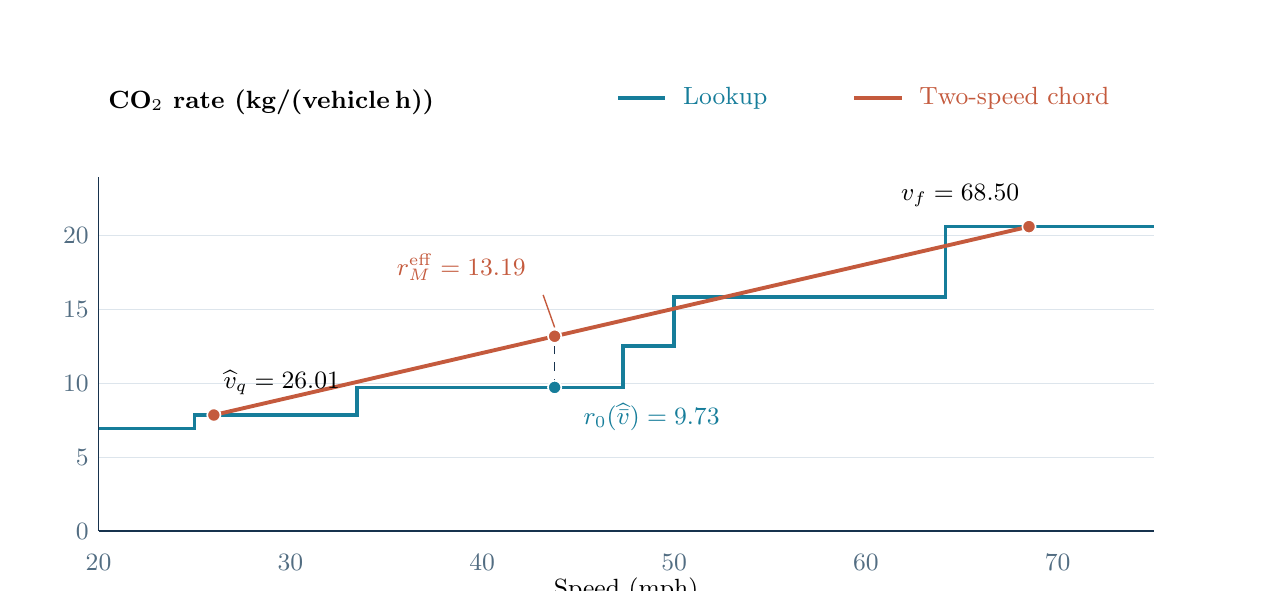
\begin{tikzpicture}[x=1cm,y=1cm,font=\small]
\path[use as bounding box] (-0.9,-0.9) rectangle (14.4,5.9);
\draw[rulegray,line width=.3pt] (0.000000,0.000000) -- (13.400000,0.000000);
\node[left,text=muted] at (0.000000,0.000000) {0};
\draw[rulegray,line width=.3pt] (0.000000,0.937500) -- (13.400000,0.937500);
\node[left,text=muted] at (0.000000,0.937500) {5};
\draw[rulegray,line width=.3pt] (0.000000,1.875000) -- (13.400000,1.875000);
\node[left,text=muted] at (0.000000,1.875000) {10};
\draw[rulegray,line width=.3pt] (0.000000,2.812500) -- (13.400000,2.812500);
\node[left,text=muted] at (0.000000,2.812500) {15};
\draw[rulegray,line width=.3pt] (0.000000,3.750000) -- (13.400000,3.750000);
\node[left,text=muted] at (0.000000,3.750000) {20};
\node[below=5pt,text=muted] at (0.000000,0.000000) {20};
\node[below=5pt,text=muted] at (2.436364,0.000000) {30};
\node[below=5pt,text=muted] at (4.872727,0.000000) {40};
\node[below=5pt,text=muted] at (7.309091,0.000000) {50};
\node[below=5pt,text=muted] at (9.745455,0.000000) {60};
\node[below=5pt,text=muted] at (12.181818,0.000000) {70};
\draw[navy] (0,0)--(13.4,0);
\draw[navy] (0,0)--(0,4.5);
\node[anchor=west,font=\small\bfseries] at (0,5.45) {CO$_2$ rate (kg/(vehicle\,h))};
\node at (6.7,-0.75) {Speed (mph)};
\draw[teal,line width=1.3pt] plot coordinates {(0.000000,1.299721) (1.218182,1.299721) (1.218182,1.472707) (3.278759,1.472707) (3.278759,1.823549) (6.658399,1.823549) (6.658399,2.350749) (7.309091,2.350749) (7.309091,2.971036) (10.754125,2.971036) (10.754125,3.865432) (13.400000,3.865432)};
\draw[rust,line width=1.4pt] (1.464406,1.472707) -- (11.816727,3.865432);
\draw[navy,dashed] (5.792524,1.823549) -- (5.792524,2.473062);
\filldraw[fill=rust,draw=white,line width=.6pt] (1.464406,1.472707) circle (2.4pt);
\filldraw[fill=rust,draw=white,line width=.6pt] (11.816727,3.865432) circle (2.4pt);
\filldraw[fill=rust,draw=white,line width=.6pt] (5.792524,2.473062) circle (2.4pt);
\filldraw[fill=teal,draw=white,line width=.6pt] (5.792524,1.823549) circle (2.4pt);
\node[anchor=south east,text=rust] at (5.548888,3.054312) {$r_M^{\eff}=13.19$};
\draw[rust,line width=.5pt] (5.646342,2.998062) -- (5.792524,2.585562);
\node[anchor=north west,text=teal] at (6.036160,1.748549) {$r_0(\widehat{\bar v})=9.73$};
\node[anchor=south west] at (1.464406,1.603957) {$\widehat v_q=26.01$};
\node[anchor=south east] at (11.816727,3.996682) {$v_f=68.50$};
\draw[teal,line width=1.3pt] (6.6,5.5)--(7.2,5.5);
\node[anchor=west,text=teal] at (7.3,5.5) {Lookup};
\draw[rust,line width=1.4pt] (9.6,5.5)--(10.2,5.5);
\node[anchor=west,text=rust] at (10.3,5.5) {Two-speed chord};
\end{tikzpicture}\end{center}
\tnote{Figure 1. The same-time rate difference for D12 I-5 north, L5N-028, AM 07:35--09:15. The vertical dashed segment is the effective-rate difference at the fitted mean speed. Rates are displayed in kg/(vehicle\,h).}

\subhead{A case with accurate delay but large two-speed error}
Observed mean speed is $44.56$ mph, fitted mean speed is $43.78$ mph, and recorded speed CV is $0.0418$. Mean-delay error is only $+5.12\%$.
Nevertheless, CO$_2$ absolute percentage error is $2.59\%$ for $S$ and $34.47\%$ for $M$.
The chord rate is $35.62\%$ above the lookup rate at the fitted mean speed.

Across all 137 episodes, the median free-flow time share is $34.8\%$, while the median free-flow emission share is $60.0\%$ for CO$_2$ and $76.3\%$ for NO$_x$.
This identifies a representation difference; it does not imply that physical free-flow travel should be removed.

\newpage
\pagetitle{How emission errors accumulate}
\subhead{Exact signed accounting}
For each episode and pollutant, the successive differences telescope:
\begin{align*}
E_A-E_O={}&(E_S-E_O)+(E_{\Sp}-E_S)\\
&+(E_R-E_{\Sp})+(E_M-E_R)+(E_A-E_M).
\end{align*}
\textbf{Table 4. Sum of each signed component divided by total reference emissions.}
\begin{center}\small
\begin{tabularx}{\linewidth}{Xrrrr}
\toprule
\textbf{Signed contribution (pp)} & \textbf{$\mathrm{CO}_2$} & \textbf{$\mathrm{NO}_x$} & \textbf{$\mathrm{CO}$} & \textbf{$\mathrm{HC}$} \\
\midrule
Observed mean-rate aggregation: $E_S-E_O$ & -4.60 & -9.56 & -2.86 & -2.51 \\
Fitted mean time and speed: $E_{\Sp}-E_S$ & +1.03 & +4.48 & -1.22 & -0.45 \\
Reconstructed speed variation: $E_R-E_{\Sp}$ & +7.78 & +15.99 & +2.28 & +2.87 \\
Two-speed allocation: $E_M-E_R$ & +16.53 & +35.63 & +3.90 & +5.08 \\
Cubic rate approximation: $E_A-E_M$ & -1.99 & -4.39 & -0.97 & -0.82 \\
Sum: total bias of $A$ & +18.76 & +42.15 & +1.13 & +4.18 \\
\bottomrule
\end{tabularx}\end{center}
\tnote{Entries are percentage points (pp). They sum to total bias, not WAPE. Cancellation occurs across steps and episodes. $R$ and $M$ share fitted vehicle-hours up to integration precision.}

\subhead{Separate vehicle-hours from effective rate}
Using $r_O^{\eff}=E_O/H_O$ and $r_M^{\eff}=E_M/\widehat H$ gives another exact identity:
\begin{align*}
E_M-E_O={}&(\widehat H-H_O)\frac{r_M^{\eff}+r_O^{\eff}}{2}\\[5pt]
&+(r_M^{\eff}-r_O^{\eff})\frac{\widehat H+H_O}{2}.
\end{align*}
\textbf{Table 5. Signed product components, normalized by total reference emissions.}
\begin{center}\small
\begin{tabularx}{\linewidth}{Xrrrr}
\toprule
\textbf{Signed contribution (pp)} & \textbf{$\mathrm{CO}_2$} & \textbf{$\mathrm{NO}_x$} & \textbf{$\mathrm{CO}$} & \textbf{$\mathrm{HC}$} \\
\midrule
Vehicle-hours component & -1.40 & -0.90 & -1.21 & -1.39 \\
Effective-rate component & +22.15 & +47.44 & +3.31 & +6.39 \\
\bottomrule
\end{tabularx}\end{center}

\notebox{The effective-rate component includes operating-speed representation, rate nonlinearity, and calibration-dependent queue speed. It is not a pure emission-function error. Both decompositions are mathematical accounting devices, not independently identified causal effects.}

\newpage
\reportgroup{3. Diagnostic checks}{3}
\pagetitle{Does correcting mean delay help?}
\subhead{A controlled diagnostic}
Hold the fitted queue speed $\widehat v_q$ and both lookup rates fixed. The two-speed rate multiplier is
\[
\Gamma=
\frac{v_f r_0(\widehat v_q)-\widehat v_q\,r_0(v_f)}{v_f-\widehat v_q}.
\]
Replace only the fitted mean delay with the observed mean delay:
\begin{align*}
E_M^{\mathrm{corr}}&=D\left[T_f r_0(v_f)+\bar w\,\Gamma\right],\\[5pt]
E_M-E_M^{\mathrm{corr}}&=D\bigl(\widehat{\bar w}-\bar w\bigr)\Gamma.
\end{align*}
\textbf{Table 6. Original and corrected errors on the same 133 feasible episodes.}
\begin{center}\small
\begin{tabular*}{\linewidth}{@{\extracolsep{\fill}}lrr@{}}
\toprule
\textbf{Pollutant} & \textbf{Original $M$ WAPE (\%)} & \textbf{Corrected $M$ WAPE (\%)} \\
\midrule
$\mathrm{CO}_2$ & 22.53 & 21.82 \\
$\mathrm{NO}_x$ & 48.27 & 46.78 \\
$\mathrm{CO}$ & 10.85 & 7.50 \\
$\mathrm{HC}$ & 12.29 & 7.61 \\
\bottomrule
\end{tabular*}\end{center}

\notebox{Correcting mean delay changes the CO$_2$/NO$_x$ errors very little, while reducing CO and HC errors substantially. Mean-delay calibration alone therefore cannot explain the CO$_2$/NO$_x$ discrepancy.}

\subhead{Which corrections are physically feasible?}
Nonnegative \emph{mean} free-flow and queue times require
\[
0\leq\bar w\leq L\left(\frac{1}{\widehat v_q}-\frac{1}{v_f}\right).
\]
This condition holds for 133 episodes. For the other four, the observed mean speed is below the fitted queue speed, so the correction would require negative free-flow time.

A stricter test retains the fitted duration and shape, rescales peak delay to $\bar w/\theta$, and checks the entire profile. Only 110 episodes then satisfy the finite-link peak constraint; the corrected arrival rates remain nonnegative in all 137.

\subhead{Independent check using already accurate delay predictions}
Among the 34 episodes with mean-delay absolute percentage error at most $10\%$, $M$ remains worse than $S$ in 31 CO$_2$ and 31 NO$_x$ cases.
CO$_2$ WAPE is $20.09\%$ versus $5.96\%$; NO$_x$ WAPE is $43.39\%$ versus $12.02\%$.
\tnote{The corrected values are counterfactual diagnostics, not newly calibrated forecasts. Table 6 uses the feasible 133-case sample on both sides; it must not be compared as though it used all 137 cases.}

\newpage
\pagetitle{Profile tests and episode-level files}
\subhead{Are flat or short episodes the explanation?}
\textbf{Table 7. CO$_2$ results by recorded-profile characteristics.}
\begin{center}\small
\begin{tabularx}{\linewidth}{Xrrr}
\toprule
\textbf{Condition} & \textbf{$N$} & \textbf{$M$ worse than $S$} & \textbf{$S$ / $M$ WAPE (\%)} \\
\midrule
Flat recorded speeds: CV $\leq0.10$ & 81 & 73/81 & 4.73 / 23.91 \\
More variable speeds: CV $>0.10$ & 56 & 48/56 & 6.45 / 21.74 \\
Short episodes: $P\leq1$ h & 26 & 23/26 & 8.06 / 20.48 \\
Longer episodes: $P>1$ h & 111 & 98/111 & 5.83 / 22.48 \\
\bottomrule
\end{tabularx}\end{center}
Flatness here means little temporal variation in the recorded five-minute speeds, using count-weighted CV. It does not establish flat individual trajectories.
In the same 81 flat episodes, CO WAPE is $6.51\%$ for $M$ versus $6.59\%$ for $S$: the finding is pollutant-specific.

No retained episode meets the illustrative shallow threshold $\bar w/T_f\leq0.25$; the minimum is $0.370$. Yet 79 episodes have mean delay at most 10 seconds because many links are short. Small absolute delay and weak relative congestion are distinct conditions.

The excess CO$_2$ absolute percentage error of $M$ over $S$ has weak rank associations with absolute trip-time percentage error ($-0.045$), speed CV ($-0.086$), and relative congestion severity ($-0.038$); the association with fitted queue speed is $-0.389$.
These are descriptive and may reflect corridor differences, not causal effects.

\subhead{Files for checking individual episodes}
\begin{center}\small
\begin{tabularx}{\linewidth}{>{\raggedright\arraybackslash}p{6.2cm}X}
\toprule
\textbf{File} & \textbf{Contents}\\
\midrule
\path{episode_review_137.csv} & Short entry point: sorted CO$_2$ error gap, pollutant-specific comparison flags, and traffic diagnostics.\\
\path{episode_calculations_137.csv} & All 137 episodes, every method total, rates, time shares, errors, and admissibility flags.\\
\path{episode_pollutant_calculations_548.csv} & Narrower format: one episode-pollutant pair per row.\\
\path{column_definitions.csv} & Calculation definitions and units for the full episode table.\\
\path{comparison_metrics.csv};\newline\path{counterfactual_metrics.csv} & Pooled scores for explicitly named, matched samples.\\
\bottomrule
\end{tabularx}\end{center}

\tnote{\textbf{Audit evidence.} All saved O/S/R/M/A totals and observed traffic targets were reproduced from the archived inputs; maximum relative discrepancy was $6.44\times10^{-13}$. An independent calculation verified the comparisons and identities. No numerical result changed during this formatting revision.}
\tnote{\textbf{Scope.} These 137 admitted cases are a selected sample of 325 detected episodes. The analysis explains agreement with a point-speed reference; it does not validate physical vehicle trajectories or measured exhaust. Source hashes and detailed checks accompany the analysis package.}
\label{LastPage}
\end{document}
